\section{Timeline for project}
This semester project can be split into 6 parts, as seen on \autoref{fig:timeline-for-project}.
There are 4 sprints in total for development of the application. 
For the PO- and process groups there is a lot of work to prepare the first sprint.
This is what we consider \textit{Pre sprint 1}.
After this, there are 4 sprints to planned the week planner application.
The process group planned the sprints such that the last sprint will end two weeks before the deadline for handing in the project.
These last two weeks will be spent on usability tests with the customers and finishing the report.
What is common for every sprint is that they follow the process guidelines previously described in \autoref{scrum-of-scrums}.

\begin{figure}[H]
    \center{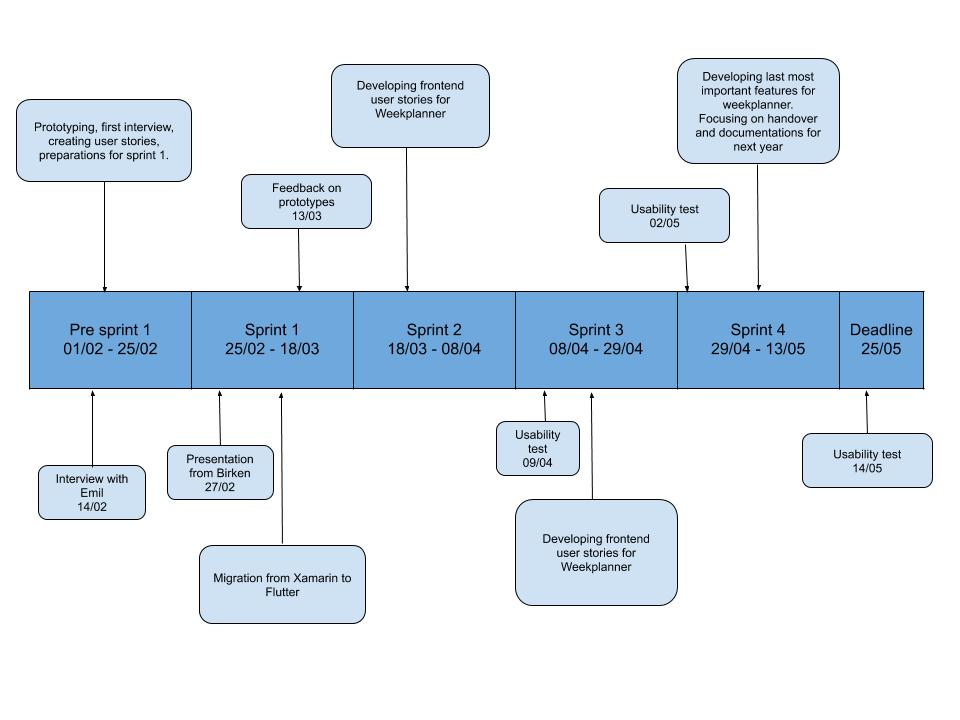
\includegraphics[width=\textwidth]
    {figures/timeline-for-entire-project.JPG}}
    \caption{\label{fig:timeline-for-project} Timeline for the project.}
\end{figure}

\noindent The light blue boxes show the highlights of what has been focused on during each sprint.

\noindent Every sprint starts with a sprint introduction where the PO group presents an introduction to the sprint.
Throughout the sprint a weekly stand up meeting is arranged, where each group can give a status update on their current progress.
Skill group meetings are arranged when the skill groups feel that they are needed.\\
Four days before a sprint ends the release preparations start.
The PO group decides which features should be included in the release during this preparation.
When the release preparations are completed, a release party is arranged where the release is presented to the rest of the groups.
This party is held to give the groups present a sense of ownership to all groups and let them see what was accomplished in the sprint. 
A sprint review is arranged after the release, followed by a sprint retrospective.

\subsubsection{Pre sprint 1}
\textit{Pre sprint 1} was where the preparation for the first sprint happened.
During this time, the groups of the GIRAF project did not fully understand the project, so it was mostly spent gathering information.
During this time the POs contact and interview customers to gain insight into what is wanted by the customers.
With these interviews, user stories and prototypes are created so that they are ready for sprint 1.
In \textit{pre sprint 1}, an interview with Emil from Egebakken was conducted. 
This interview is described in \autoref{interview-with-emil}.
The process group focuses on establising the process guidelines, while the development groups are researching the existing codebase.

\subsubsection{Sprint 1}
A presentation from the kindergarten Birken was given on February 27th.
This presentation is described in \autoref{presentation-from-birken}.
The focus of this sprint started out as fixing bugs and making the application more stable.
It turned out that there were a lot of problems with the frontend with Xamarin, and it was decided that the frontend should be migrated to Flutter during an extraordinary meeting involving most participants of the project. \\
The pros and cons of the decision are described in \autoref{change-of-framework}.
This also resulted in the PO group needing to look into the user stories, as new user stories for previously implemented features needed to be implemented again and many of the old user stories had to gain a lower priority.
A meeting was planned with the customers on March 13th to get feedback on the prototypes. 
This interview resulted in some of the prototypes getting reworked to better fit the customers needs.

\subsubsection{Sprint 2}
As there was no release at the end of sprint 1 due to the decision to migrate to Flutter, several of the user stories assigned in Sprint 1 were not completed and as a result of this, there was no reason to conduct a usability test in sprint 1.
Instead, sprint 2 was mostly spent developing user stories planned in sprint 1 and some additional user stories for sprint 2.
During this sprint the PO group also implemented some user stories, which are described in \autoref{our-assigned-user-stories-sprint-2}
At the end of this sprint the first release was completed.

\subsubsection{Sprint 3}
There were still some leftover user stories from sprint 1 and sprint 2, which were not completed due to some dependencies. 
At this point the project is starting to have a some of the most essential features implemented, but still a needing a lot of features before it being useable. 
This sprint focused mostly on implementing user stories.
However, there were also developed new prototypes during this sprint.
This sprint ended with a usability test which are described in \todo{ref til rasmus' lort}

\subsubsection{Sprint 4}
As sprint 4 was our final sprint, the sprint mostly focused on finishing the work that was not completed in the previous sprints and developing the most important user stories to have a minimal viable product.
The PO group and process group did not implement user stories in this sprint, because they focused on documentation and making the handover to next year students as thorough as possible.
In the end of the sprint the final usability test was conducted.
The purpose of this usabiltiy test was to get a better understanding of what the application was lacking and what the next year students should focus on.

\subsubsection{Deadline}
All development on the weekplanner ended May 13th, after this all groups were expected to only focus on finishing their report.
The PO group still needed to finish some documentation for next year, as the last usability test was held on May 14th.
Project hand in was on May 28th.
